% LLNCS macro package for Springer Computer Science proceedings;
% This is samplepaper.tex, a sample chapter demonstrating the
% Version 2.20 of 2017/10/04
%
\documentclass{llncs}

% ─── Encoding & Fonts ─────────────────────────────────────────────────────────
\usepackage[utf8]{inputenc}
\usepackage{lmodern}              % Scalable font

% ─── Mathematics ──────────────────────────────────────────────────────────────
\usepackage{amsmath}
% \usepackage{amsthm}             % Uncomment if theorem environments needed

% ─── Tables ───────────────────────────────────────────────────────────────────
\usepackage{array}
\usepackage{multirow}
\usepackage{tabularx}
\usepackage{booktabs}
\usepackage{longtable}
\usepackage{arydshln}             % Dashed lines in tables
\usepackage{adjustbox}

% ─── Figures & Floats ─────────────────────────────────────────────────────────
\usepackage{graphicx}
\usepackage{float}

% ─── Algorithms ───────────────────────────────────────────────────────────────
\usepackage{algorithm, algorithmic}
\usepackage{algpseudocode}

% ─── Layout & Formatting ──────────────────────────────────────────────────────
\usepackage{indentfirst}
\usepackage{seqsplit}

% ─── Patching & Utilities ─────────────────────────────────────────────────────
\usepackage{etoolbox}
\usepackage{regexpatch}

% ─── Symbols & Icons ──────────────────────────────────────────────────────────
\usepackage{marvosym}             % \Letter and other symbols

% ─── References & Links ───────────────────────────────────────────────────────
\usepackage{cite}
\usepackage{hyperref}
% \renewcommand\UrlFont{\color{blue}\rmfamily}  % Springer eBook URL style
% \bibliographystyle{splncs04}

% ─── Custom Commands ──────────────────────────────────────────────────────────
\newcommand{\quo}[1]{``#1''}
\newcommand{\mycomment}[1]{}
\newcommand{\Indent}{\hspace{1.5em}}
\newcommand{\EndIndent}{}

\makeatletter
\newcommand{\printfnsymbol}[1]{%
  \textsuperscript{\@fnsymbol{#1}}%
}
\makeatother

\begin{document}
% \title{Developing a Multi-Objective Evolutionary Algorithm for Disaster Relief Hub Network Design}
% \title{Modeling and solving the disaster relief hub network design problem: A case of Central Coastal Vietnam}
\title{Humanitarian Logistics Hub Network Design Under Uncertainty: A Multi-Objective Model and Priority-Based Genetic Algorithm for Central Coastal Vietnam}

% \titlerunning{MOEA for Disaster Relief HLP}
\titlerunning{Multi-Objective Flood Relief Hub Network Design via PB-NSGA}
% If the paper title is too long for the running head, you can set
% an abbreviated paper title here
%
\author{
    Phu-Quy Le-Tang\inst{1} \and
    Quang-Vu Nguyen \inst{1} \and
    Sunarin Chanta \inst{2} \thanks{Corresponding author.}
}

    %
\authorrunning{Le Tang Phu Quy et al.}
    % First names are abbreviated in the running head.
    % If there are more than two authors, 'et al.' is used.
    %
\institute{
    The University of Danang, Vietnam - Korea University of Information and Communication Technology  
    \and King Mongkut's University of Technology North Bangkok \\
    \email{
        quyltp.22git@vku.udn.vn,
        nqvu@vku.udn.vn,
        sunarin.c@itm.kmutnb.ac.th
    }
}
%
\maketitle              % typeset the header of the contribution
%
\begin{abstract}

Natural disasters severely disrupt transportation infrastructure, heavily complicating search and rescue (SAR) operations. Existing humanitarian logistics models often fail to capture these dynamic disruptions and the non-linear escalation of human suffering. To address this gap, we propose a two-stage stochastic Multi-Objective Incomplete Hub Location Network Design Problem (MO-IHLNDP). Our model simultaneously minimizes expected logistics costs -- utilizing Daganzo's Continuous Approximation for scalable last-mile routing -- and the expected maximum deprivation cost to enforce social equity. To solve this NP-hard problem, we develop a Priority-Based Non-dominated Sorting Genetic Algorithm II (PB-NSGA-II). Extensive computational experiments on standard benchmarks (AP, TR81) validate the algorithm's efficiency. Furthermore, a detailed case study of the flood-prone Vu Gia -- Thu Bon river basin provides crucial managerial insights. The results highlight the necessity of dynamically adapting multi-modal network topologies to maintain resilience under extreme disaster scenarios.
\keywords{Humanitarian Logistics \and Disaster relief \and Hub location problem \and Multi-objective Evolutionary Algorithm.}
\end{abstract}

\section{Introduction}
\subsection{Problem}

Natural disasters are becoming increasingly frequent and violent, continuously exposing supply chain weaknesses and causing massive economic losses \cite{ASEAN2021, CDP2025}.
As a highly vulnerable coastal country, Vietnam has witnessed unprecedented extreme weather events.
In 2025 alone, a relentless sequence of typhoons and record-breaking floods in Central Vietnam resulted in massive fatalities and an estimated 98.7 trillion VND in economic losses \cite{VOV2025, HanoiTimes2025}.

There were many great challenges in humanitarian operations during this period.
Most critically, national logistics infrastructure suffered severe disruption: the North-South Railway was paralyzed by track erosion and submersion, forcing the cancellation of 170 trains~\cite{HanoiTimes2025}, while key arteries such as National Highway 1 were severed by landslides, isolating communities for days~\cite{ReliefWeb2020}.
These events demonstrate that during a major catastrophe, the assumption of a fully connected transport network is fundamentally flawed -- the physical network becomes \quo{incomplete}, characterized by broken links and isolated nodes.
Compounding this, resource scarcity arising from poor planning and uncertain supply and demand further strains relief efforts.
Disaster management involves four phases: mitigation, preparedness, response, and recovery~\cite{altay2006or}; Disaster Relief Network Design (DRND) bridges the preparedness and response phases by optimizing facility locations and relief routing.

\subsection{Related Works}

\textbf{Humanitarian logistics and facility location.}
Humanitarian logistics differs fundamentally from its commercial counterpart in that speed and equity dominate over cost minimisation~\cite{van2006humanitarian, kovacs2007humanitarian}.
A comprehensive review of humanitarian facility location under uncertainty~\cite{donmez2021humanitarian} identifies stochastic programming and robust optimisation as the dominant paradigms, while Boonmee et al.~\cite{boonmee2017facility} document the growing need for models that jointly capture disruption, uncertainty, and equity.
Critically, Holgu{\'i}n-Veras et al.~\cite{HolguinVeras2012, holguin2013appropriate} argued that purely cost-based objectives neglect social welfare, and proposed \emph{deprivation cost} -- an exponential penalty on victim waiting time -- as the appropriate humanitarian objective.

\textbf{Hub location and incomplete networks.}
Hub-and-spoke structures consolidate flows efficiently and have been studied extensively since Campbell's seminal formulations~\cite{campbell1994integer}.
For disaster settings, the \emph{incomplete} hub network -- in which infrastructure damage severs inter-hub arcs -- is a more realistic topology than the classical fully-connected graph~\cite{alumur2009incomplete}.
Sangsawang and Chanta~\cite{sangsawang2020capacitated} proposed a pioneering flood-specific hub location model, a single-objective deterministic formulation for Thailand, establishing that hub-and-spoke structures yield measurable gains in relief distribution efficiency.
Multi-modal hub networks further address the heterogeneous transport modes (road, waterway, air) that characterise disaster response~\cite{Li2023}.

\textbf{Stochastic and robust optimisation for relief networks.}
The two-stage stochastic programming framework naturally separates pre-disaster strategic decisions from post-disaster recourse~\cite{elci2018chance, tofighi2016humanitarian}.
Under demand and supply uncertainty, robust formulations~\cite{Yahyaei2019, sun2022novel} and prepositioning models~\cite{abazari2021prepositioning} have been shown to outperform deterministic baselines.
Disruption of transportation infrastructure compounds this uncertainty by rendering pre-planned routes infeasible~\cite{salman2015emergency}, a condition endemic to Central Vietnam's flood disasters.

\textbf{Multi-objective evolutionary algorithms.}
NSGA-II~\cite{deb2002fast} is the standard framework for multi-objective
combinatorial problems in humanitarian logistics, owing to its parameter-free
Pareto ranking and elitist selection.
Zhou et al.~\cite{Zhou2017} applied a multi-objective evolutionary algorithm
to multi-period dynamic emergency resource scheduling under uncertain road
networks, demonstrating the effectiveness of population-based search when
scenario-dependent decisions are coupled to shared strategic variables.
Li et al.~\cite{Li2023} designed a bi-objective multimodal hub-and-spoke
network for emergency relief using a meta-heuristic approach, showing that
problem-specific customized operators are essential for maintaining feasibility
across complex network topologies.

\textbf{Research gap and contributions.}
No existing work simultaneously addresses incomplete hub network design, two-stage stochastic programming, multi-objective humanitarian objectives (logistics cost and deprivation cost), and a flood-disaster case study.
Sangsawang and Chanta~\cite{sangsawang2020capacitated} is the closest precedent, yet it is deterministic and single-objective.
The present paper closes this gap by proposing MO-IHLNDP -- a two-stage stochastic multi-objective incomplete hub location model integrating Daganzo's CA for last-mile cost estimation -- and PB-NSGA-II, a priority-based~\cite{gen2006priority} evolutionary algorithm that efficiently reconstructs second-stage decisions across flood scenarios in Central Coastal Vietnam.

\mycomment{
\subsection{Related Works}

The design of disaster relief networks differs fundamentally from commercial logistics. Commercial models prioritize profit maximization. Humanitarian logistics prioritizes human lives and rapid response \cite{van2006humanitarian}. Facility location is a critical component of disaster preparedness. A comprehensive review by Boonmee et al. \cite{boonmee2017facility} highlights the growing need for facility location models under severe uncertainty. 

\textbf{Disruption and Network Design.} Disasters often cause severe infrastructure disruptions. Standard network models fail when paths become unavailable. Yahyaei and Bozorgi-Amiri \cite{Yahyaei2019} addressed this by proposing a robust reliable network design. They integrated shelter and supply facility locations under disruption risks. Similarly, Hasani and Mokhtari \cite{Hasani2019} proposed an integrated relief network model for Iran. They modeled dynamic uncertainty and employed multi-objective optimization. However, embedding exact routing sequences into these network designs creates highly intractable Location-Routing Problems (LRP).

\textbf{Continuous Approximation.} To circumvent the NP-hard complexity of exact routing, researchers utilize approximations. Daganzo \cite{daganzo2005logistics} pioneered the Continuous Approximation (CA) method. CA estimates last-mile routing costs using spatial densities rather than explicit node-to-node sequences. This technique drastically reduces computational burden. It allows large-scale network models to remain tractable. Our model adopts this CA framework to estimate evacuation costs efficiently.

\textbf{Deprivation Cost and Social Equity.} Traditional objective functions usually minimize pure logistics costs or average travel times. Holguín-Veras et al. \cite{holguin2013appropriate} argued that linear time penalties neglect social equity. They introduced the concept of deprivation cost. It applies an exponential penalty function to waiting times. This mathematically captures the non-linear escalation of human suffering during disasters. Incorporating deprivation cost forces optimization models to distribute resources equitably. It prevents the marginalization of isolated distress clusters.

\textbf{Solution Approaches.} Disaster relief models often involve multiple conflicting objectives. Meta-heuristics are highly preferred for these problems. NSGA-II \cite{deb2002fast} is a standard and robust evolutionary framework. It utilizes non-dominated sorting and crowding distance to find Pareto-optimal solutions. Recent studies frequently adapt NSGA-II for humanitarian operations. 

\textbf{Research Gap and Our Contribution.} Existing literature contains a significant gap. Very few studies integrate incomplete hub networks, Daganzo's continuous approximation, and exponential deprivation costs under a two-stage stochastic framework. Solving such a combined model is computationally prohibitive for exact solvers. Our study addresses this gap. We formulate the MO-IHLNDP and propose a meta-heuristic algorithm named Priority-Based NSGA-II, which can handle large-scale instances effectively.


\subsection{My Draft}
\textbf{I rethought carefully. I'd develop a more manageable and approachable model}.
\begin{figure}
    \centering
    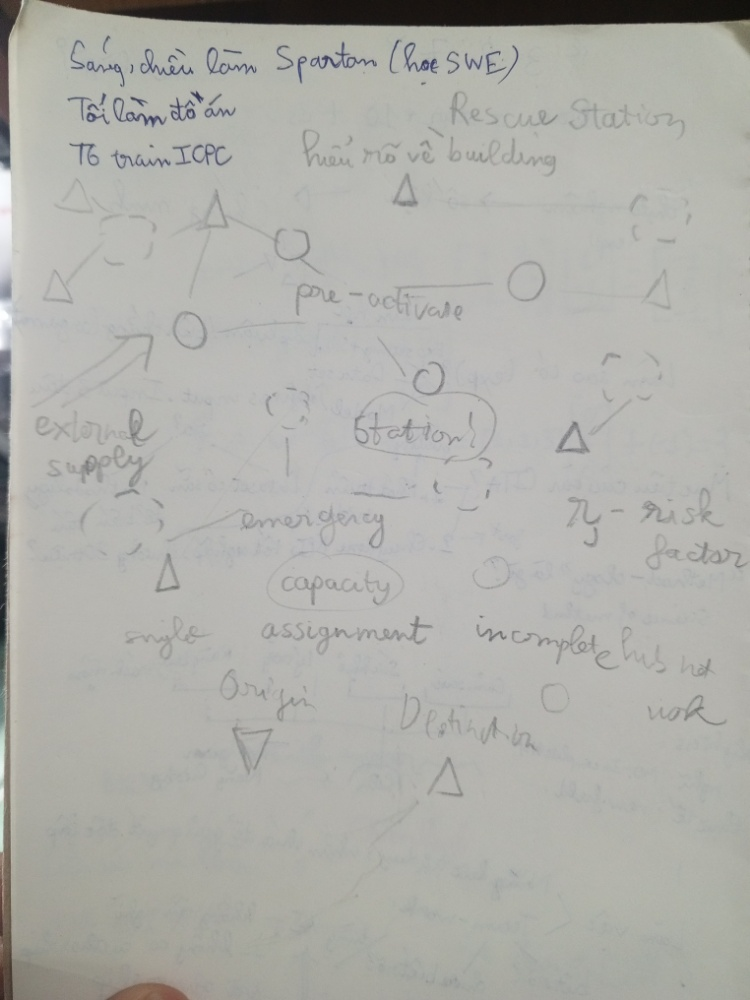
\includegraphics[width=0.5\linewidth]{model-illustration-sketch.png}
    \caption{Illustration of the model}
    \label{fig:placeholder}
\end{figure}
\begin{figure}
    \centering
    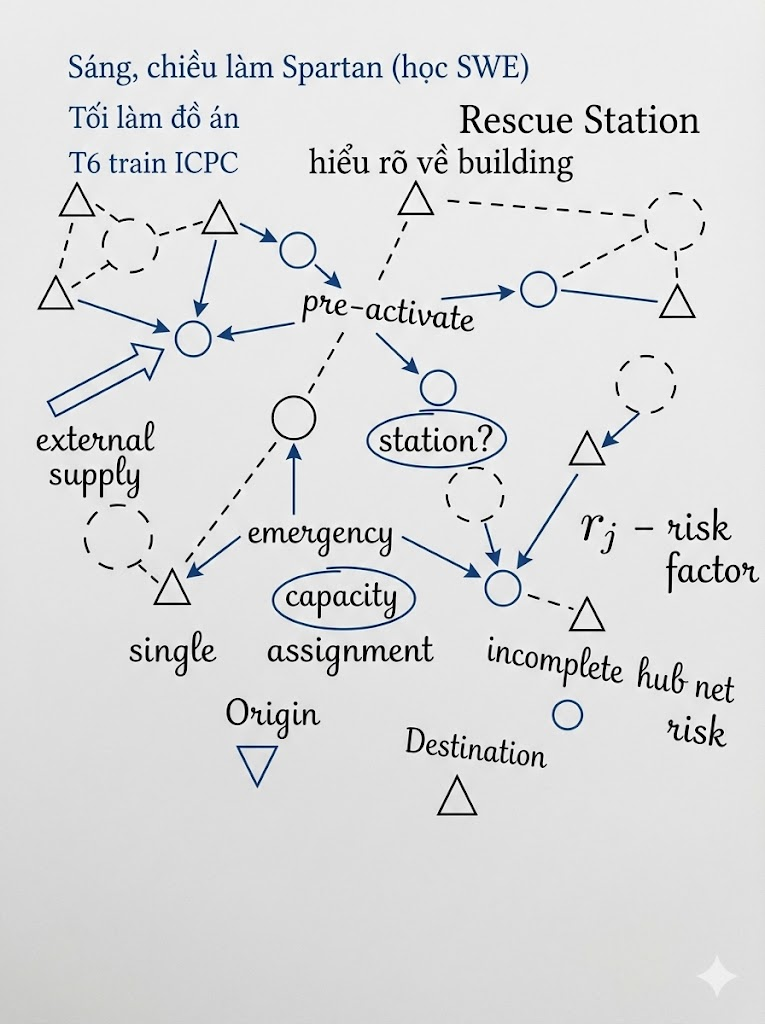
\includegraphics[width=0.5\linewidth]{model-illus-ai.png}
    \caption{AI-generated illustration}
    \label{fig:placeholder}
\end{figure}
}

\section{Problem Description and Mathematical Model}

To design an efficient disaster relief network (DRND) for flood disaster response in Central Vietnam, we frame the problem as a multi-objective incomplete hub location network design problem (MO-IHLNDP) -- the capacitated, single-allocation variant of the HLP. The network comprises three main components: origins, hubs, and demands. Hubs refer to rescue stations of two kinds: the first is established in advance of the disaster, strategically positioned and pre-inventoried with amenities; the second is opened dynamically during response, prioritizing approachability to affected areas. \textbf{Demands} refer to victim groups discovered progressively during operations, while \textbf{origins} represent both government-planned forces and spontaneous volunteers.

From a practical standpoint, DRND involves two critical uncertainty factors. First, infrastructure disruption -- damaged roads and buildings -- can disable pre-programmed plans, urging the need for a dynamic solution~\cite{Yahyaei2019}. Second, the exact locations of demands, the total number of victims, and the availability of origins are all highly uncertain during rescue operations~\cite{tofighi2016humanitarian}. To account for these, we employ a two-stage stochastic programming approach across multiple scenarios, each assigning a specific risk factor per area, and assume that SAR operations rely heavily on dynamic external supply sources, as pre-positioned hubs may not fully satisfy uncertain demands under extreme scenarios.

Finally, the model places strong emphasis on \textit{social equity} by integrating the deprivation cost~\cite{holguin2013appropriate}, and adopts Daganzo's continuous approximation~\cite{daganzo2005logistics} to obtain a tractable yet robust estimate of rescue time from each hub to its assigned demand points.

\subsection{Sets and Indices}
\noindent
\begin{tabular}{l p{0.85\textwidth}}
$\mathcal{H}, \mathcal{I}, \mathcal{J}$ & Set of candidate hubs ($k, h$), demand nodes ($i$), and  origins ($j$) \\
$\mathcal{S}, \mathcal{M}$ & Set of disaster scenarios ($s$) and transportation modes ($m$) \\
$\mathcal{V}$ & Set of all nodes ($u,v$) representing the area in question, $\mathcal{V} = \mathcal{H} \cup \mathcal{I} \cup \mathcal{J}$ \\
\end{tabular}

\subsection{Parameters}

\noindent \textbf{First-Phase Parameters (Strategic Planning)} \\
\begin{tabular}{l p{0.85\textwidth}}
$F_k$ & Fixed cost to establish hub $k$ of the first type (before the disaster) \\
$c_k, \kappa_k$ & Unit holding cost and capacity limit for inventory at hub $k$ \\
$\alpha, \chi, M$ & Discount factor for economies of scale, max acceptable risk threshold, and Big-M constant \\
$C_{uvm}, \tau_{uvm}$ & Unit transportation cost and estimated travel time from node $u$ to $v$ via mode $m$ \\
$C_m, Q_m$ & Unit local routing cost and transportation capacity for vehicle mode $m$ \\
$\gamma$ & Conversion factor (average amount of relief items required per evacuated person) \\
\end{tabular}

% \vspace{0.2cm}
\noindent \textbf{Second-Phase Parameters (Disaster Response, Scenario $s$)} \\
\begin{tabular}{l p{0.85\textwidth}}
$\pi_s$ & Probability of scenario $s$ \\
$F_{ks}^{a}$ & Fixed cost to establish hub $k$ of the second type (reactive) in scenario $s$ \\
$\tau_{ks}$ & Processing time for each rescue round trip at hub $k$ in scenario $s$ \\
$a_{uvms}$ & Accessibility of arc $(u,v)$ via mode $m$ in scenario $s$ (1 if traversable, 0 otherwise) \\
$r_{us}, \lambda_{is}$ & Risk index of node $u$, and deprivation sensitivity coefficient for demand $i$ in scenario $s$ \\
$D_{is}, O_{js}$ & Demand (number of people to evacuate) at $i$, and relief items provided at origin $j$ in scenario $s$ \\
$c_{jks}$             & Pre-computed cheapest transport cost from origin $j$ to hub $k$ in scenario $s$:
                        $c_{jks} = \min_{m \in \mathcal{M} \mid a_{jkms}=1} C_{jkm}$, ($+\infty$ if no available mode) \\
$\Theta_{kis}$ & Pre-computed CA routing cost to execute the evacuation from grid $i$ to hub $k$ in scenario $s$ \\
$\Phi, \eta, A_i$ & Daganzo's circuity factor, average group size per distress location, and area of grid cell $i$ \\
\end{tabular}

\subsection{Decision Variables}
\noindent
\begin{tabular}{l p{0.85\textwidth}}
$x_{k} \in \{0,1\}$ & 1 if hub $k$ is established as the first type (planned), 0 otherwise \\
$y_{ks} \in \{0,1\}$ & 1 if hub $k$ is established as the second type (reactive) in scenario $s$, 0 otherwise \\
$z_{iks} \in \{0,1\}$ & 1 if demand $i$ is assigned to be evacuated to hub $k$ in scenario $s$, 0 otherwise \\
$z_{jks} \in \{0,1\}$ & 1 if origin $j$ supplies hub $k$ in scenario $s$, 0 otherwise \\
$q_{k} \ge 0$ & Amount of relief items inventoried at hub $k$ \\
$f_{khms} \ge 0$ & Lateral trans-shipment flow volume from hub $k$ to hub $h$ via mode $m$ in scenario $s$ \\
\end{tabular}

\subsection{Objectives}
\textbf{Objective 1: Minimize Total Expected Logistics Cost ($Z_1$)}

\begin{equation} \label{eq:obj1}
\begin{aligned}
    \text{Min } Z_1 = & \underbrace{\sum_{k \in \mathcal{H}} F_k x_k + \sum_{k \in \mathcal{H}} c_k q_k}_{\text{Pre-disaster strategic costs}} \\
    & + \sum_{s \in \mathcal{S}} \pi_s \Bigg[ \underbrace{\sum_{k \in \mathcal{H}} F_{ks}^a y_{ks}}_{\text{Reactive setup}} 
    + \underbrace{\sum_{j \in \mathcal{J}} \sum_{k \in \mathcal{H}} c_{jks} \cdot O_{js} z_{jks}}_{\text{Origin to Hub supply flow}} \\
    % + \underbrace{\sum_{j \in \mathcal{J}} \sum_{k \in \mathcal{H}} \left( \min_{m \in \mathcal{M} \mid a_{jkms}=1} C_{jkm} \right) O_{js} z_{jks}}_{\text{Origin to Hub supply flow}} \\
    % + \underbrace{\sum_{j \in \mathcal{J}} \sum_{k \in \mathcal{H}} \sum_{m \in \mathcal{M}} C_{jkm} O_{js} z_{jks}}_{\text{Origin to Hub supply flow}} \\
    & + \underbrace{\sum_{k \in \mathcal{H}} \sum_{h \in \mathcal{H}} \sum_{m \in \mathcal{M}} \alpha C_{khm} f_{khms}}_{\text{Inter-hub lateral trans-shipment}} 
    + \underbrace{\sum_{k \in \mathcal{H}} \sum_{i \in \mathcal{I}} \Theta_{kis} z_{iks}}_{\text{Grid-based Last-Mile CA}} 
    \Bigg]
\end{aligned}
\end{equation}

Objective $Z_1$ minimizes the total expected logistics cost, balancing pre-disaster investments against reactive setups and transportation costs. To have an accurate estimation of last-mile evacuation cost while keeping the model simple, we adopted Daganzo's Continuous Approximation \cite{daganzo2005logistics}. The region of interest is partitioned via spatial discretization, and the demands are aggregated on a grid basis. The routing cost $\Theta_{kis}$ is pre-computed as a parameter:
\begin{equation*} \label{eq:daganzo_theta}
    \Theta_{kis} = \min_{m \in \mathcal{M}} \left( 2 \cdot C_{kim} \cdot \lceil D_{is}/Q_m \rceil + C_{m} \cdot \Phi \sqrt{\lceil D_{is}/\eta \rceil \cdot A_i} \right)
\end{equation*}

\textbf{ Objective 2: Minimize Expected Maximum Deprivation Cost ($Z_2$)}

% Formula: max (s over S) (sum i over I) IS CHANGED TO avg (s over S) (max i over I)
% \begin{equation} \label{eq:obj2}
% \text{Min } Z_2 = \max_{s \in \mathcal{S}} \left( \sum_{i \in \mathcal{I}} D_{is} \cdot \left( e^{\lambda_{is} \cdot \Omega_{is}} - 1 \right) \right)
% \end{equation}

\begin{equation} \label{eq:obj2}
    \text{Min } Z_2 = \sum_{s \in \mathcal{S}} \pi_s \left( \max_{i \in \mathcal{I}} \left[ D_{is} \cdot \left( e^{\lambda_{is} \cdot \Omega_{is}} - 1 \right) \right] \right)
\end{equation}

The second objective ensures social equity by minimizing the expected maximum deprivation cost across all scenarios. Based on Holguín-Veras et al. \cite{holguin2013appropriate}, $Z_2$ adopts an exponential function to penalize long waiting times ($\Omega_{is}$) for victims. Furthermore, it forces the model to distribute resources evenly, ensuring overall low delay time for everyone.

\begin{equation*} \label{eq:waiting_time}
\Omega_{is} = \sum_{k \in \mathcal{H}} z_{iks} \left( \tau_{ks} + 2 \cdot \min_{m \in \mathcal{M}} \tau_{kim} \right)
\end{equation*}

The sensitivity coefficient $\lambda_{is}$ is proportional to the risk index $r_{is}$ ($\lambda_{is} = \lambda_0(1 + r_{is})$), effectively prioritizing vulnerable populations. Although $Z_2$ introduces non-linearity, our meta-heuristic solution approach can directly evaluate it as a fitness function. For linearization into a Mixed-Integer Linear Programming (MILP) form, one can exploit the single-allocation property ($\sum_{k \in \mathcal{H}} z_{iks} = 1$).

\subsection{Constraints}

The complete MO-IHLNDP model is formally stated as follows:

\allowdisplaybreaks
\begin{align}
    \text{Minimize } \quad & Z_1, Z_2 \nonumber \\
    \text{subject to} \quad & \text{Constraints } \eqref{eq:hub_type} - \eqref{eq:nonneg_vars} \nonumber \\
    x_k + y_{ks} & \le 1 \quad \forall k \in \mathcal{H}, s \in \mathcal{S} \label{eq:hub_type} \\
    q_k & \le \kappa_k \cdot x_k \quad \forall k \in \mathcal{H} \label{eq:hub_inv_cap} \\
    r_{ks} \cdot (x_k + y_{ks}) & \le \chi \quad \forall k \in \mathcal{H}, s \in \mathcal{S} \label{eq:hub_safety} \\
    \sum_{k \in \mathcal{H}} z_{iks} & = 1 \quad \forall i \in \mathcal{I}, s \in \mathcal{S} \label{eq:single_alloc_demand} \\
    \sum_{k \in \mathcal{H}} z_{jks} & = 1 \quad \forall j \in \mathcal{J}, s \in \mathcal{S} \label{eq:single_alloc_origin} \\
    z_{iks} & \le x_k + y_{ks} \quad \forall i \in \mathcal{I}, k \in \mathcal{H}, s \in \mathcal{S} \label{eq:valid_assign_demand} \\
    z_{jks} & \le x_k + y_{ks} \quad \forall j \in \mathcal{J}, k \in \mathcal{H}, s \in \mathcal{S} \label{eq:valid_assign_origin} \\
    z_{iks} & \le \sum_{m \in \mathcal{M}} a_{ikms} \quad \forall i \in \mathcal{I}, k \in \mathcal{H}, s \in \mathcal{S} \label{eq:path_demand} \\
    z_{jks} & \le \sum_{m \in \mathcal{M}} a_{jkms} \quad \forall j \in \mathcal{J}, k \in \mathcal{H}, s \in \mathcal{S} \label{eq:path_origin} \\
    f_{khms} & \le M \cdot a_{khms} \quad \forall k, h \in \mathcal{H}, m \in \mathcal{M}, s \in \mathcal{S} \label{eq:trans_path} \\
    % \sum_{i \in \mathcal{I}} \gamma D_{is} z_{iks} + \sum_{h \in \mathcal{H}} \sum_{m \in \mathcal{M}} f_{khms} & \le q_k + \sum_{j \in \mathcal{J}} O_{js} z_{jks} + \sum_{h \in \mathcal{H}} \sum_{m \in \mathcal{M}} f_{hkms} \quad \forall k \in \mathcal{H}, s \in \mathcal{S} \label{eq:flow_balance} \\
    \begin{split}
        \sum_{i \in \mathcal{I}} \gamma D_{is} z_{iks} + \sum_{h \in \mathcal{H}} \sum_{m \in \mathcal{M}} f_{khms} & \le q_k + \sum_{j \in \mathcal{J}} O_{js} z_{jks} \\
        & \quad + \sum_{h \in \mathcal{H}} \sum_{m \in \mathcal{M}} f_{hkms} \quad \forall k \in \mathcal{H}, s \in \mathcal{S} 
    \end{split} \label{eq:flow_balance} \\
    q_k + \sum_{j \in \mathcal{J}} O_{js} z_{jks} + \sum_{h \in \mathcal{H}} \sum_{m \in \mathcal{M}} f_{hkms} & \le \kappa_k \cdot (x_k + y_{ks}) \quad \forall k \in \mathcal{H}, s \in \mathcal{S} \label{eq:throughput_cap} \\
    x_k, y_{ks}, z_{iks}, z_{jks} & \in \{0, 1\} \quad \forall i, j, k, s \label{eq:binary_vars} \\
    q_k, f_{khms} & \ge 0 \quad \forall k, h, m, s \label{eq:nonneg_vars}
\end{align}

Constraints \eqref{eq:hub_type} define
the hub establishment. For planned hubs, inventory is bounded by physical capacity \eqref{eq:hub_inv_cap}, while the reactive hubs are required to be placed within safe zones \eqref{eq:hub_safety}.
Constraints \eqref{eq:single_alloc_demand}-\eqref{eq:path_origin} rigorously enforce the single-allocation property to active hubs via available links. 
Constraint \eqref{eq:trans_path} restricts flow to be trans-shipped on intact paths. 
Constraints \eqref{eq:flow_balance} and \eqref{eq:throughput_cap} maintain flow conservation and capacity limits. Specifically, \eqref{eq:flow_balance} ensures that total supply, comprising inventory ($q_k$), external origins ($O_{js}$), and incoming flows -- satisfies both victim demand (converted by $\gamma$) and outgoing trans-shipments.
Variable domains are defined in \eqref{eq:binary_vars}-\eqref{eq:nonneg_vars}.

\section{Proposed Algorithm: PB-NSGA}

The MO-IHLNDP is NP-hard, as its single-objective, single-scenario relaxation subsumes the uncapacitated facility location problem~\cite{mirchandani1990discrete}. 
We therefore propose \textbf{PB-NSGA} (Priority-Based Nondominated Sorting Genetic Algorithm), which embeds the NSGA-II framework~\cite{deb2002fast} with a custom heuristic decoder.

\subsection{Chromosome Encoding Scheme}

Each chromosome $\mathbf{C} = (\mathbf{X}, \mathbf{R}, \mathbf{A}, \mathbf{W})$ consists of four segments. The binary vector $\mathbf{X} \in \{0,1\}^{|\mathcal{H}|}$ determines planned hub establishment. The continuous vector $\mathbf{R} \in [0,1]^{|\mathcal{H}|}$ defines the inventory fill fraction, setting $q_k = R_k \cdot \kappa_k$. The integer vector $\mathbf{A} \in \{0,\ldots,|\mathcal{H}|-1\}^{|\mathcal{I}|}$ encodes the preferred anchor hub for each demand $i$. The continuous vector $\mathbf{W} \in [0,1]^6$ contains six heuristic weights governing the decoder: $w_0$ and $w_3$ dictate demand sorting priority by urgency ($\lambda \cdot D$) and isolation; $w_1$, $w_2$, $w_4$ score candidate hubs by travel time, residual inventory, and preference for planned over reactive hubs; $w_5$ controls conservatism towards opening new reactive hubs.

\subsection{Priority-Based Decoding Heuristic}
\label{sec:decoder}

The decoder is invoked once per chromosome per scenario $s \in \mathcal{S}$, reconstructing all second-stage decisions from $\mathbf{C}$ in four steps.

\textbf{Step 1 -- Initialisation.} Planned hubs with $X_k = 1$ and $r_{ks} \le \chi$ are activated with pre-positioned inventory $q_k = R_k \cdot \kappa_k$; if none qualify, the safest hub is forced active. The proximity order $\pi_k$, ranking all hubs by ascending distance from anchor hub $k$, is pre-computed once.

\textbf{Step 2 -- Demand Prioritisation.} Each demand node $i$ receives a composite score
\begin{equation}
    \text{Score}_i = w_0\,\widetilde{\text{urgency}}_i + w_3\,\widetilde{\text{isolation}}_i - w_1\,\widetilde{\text{dist}}_i + \varepsilon_i,
    \label{eq:demand_score}
\end{equation}
where urgency $= \lambda_{is}D_{is}$, isolation $= 1/|\mathcal{H}_{\text{act},i}|$, and dist $=$ minimum travel time to any active hub, each normalised to $[0,1]$; $\varepsilon_i \sim \mathcal{N}(0,\sigma)$ prevents premature convergence. Demands are processed in descending score order.

\textbf{Step 3 -- Tiered Hub Assignment.} For each demand $i$, the trial order follows $\pi_{A_i}$. Let $K = \max(1, \lceil w_5 \cdot |\mathcal{H}| \rceil)$. \textit{Pass 1} selects the hub maximising $\text{HubScore}(k) = w_1/\tau_{ikm^*} + w_2 \cdot \text{residual}_k + w_4 \cdot \mathbf{1}[X_k=1]$ among the $K$ closest-to-anchor hubs that are active, reachable, and have positive residual inventory. If Pass~1 fails, \textit{Pass~2} assigns $i$ to the first active reachable hub from the remaining candidates (capacity violation permitted). If both passes fail, a \textit{reactive fallback} opens the nearest safe inactive hub at cost $F^a_{ks}$; irrecoverable infeasibility accumulates as constraint violation.

\textbf{Step 4 -- Supply Routing and Objective Accumulation.} Origins are greedily assigned to the most under-supplied active hub. Surplus inventory is redistributed via inter-hub trans-shipment with discount $\alpha$. $Z_1$ and $Z_2$ are accumulated as probability-weighted expectations over all $s \in \mathcal{S}$. Algorithm~\ref{alg:decoder} formalises Steps 1--4.

\begin{algorithm}[htbp]
\caption{Priority-Based Decoder (single scenario $s$)}
\label{alg:decoder}
\begin{algorithmic}[1]
\REQUIRE Chromosome $\mathbf{C}=(\mathbf{X},\mathbf{R},\mathbf{A},\mathbf{W})$, scenario $s$, instance data
\ENSURE $(Z_1^s,\,Z_2^s,\,\text{CV}^s)$
\STATE Activate $\mathcal{H}_{\text{act}}\leftarrow\{k:X_k\!=\!1,\;r_{ks}\!\le\!\chi\}$; set $q_k\!\leftarrow\!R_k\kappa_k$
\IF{$\mathcal{H}_{\text{act}}=\emptyset$} \STATE Force-activate $\arg\min_k r_{ks}$ among $\{k:X_k\!=\!1\}$ \ENDIF
\STATE Score each demand $i$ by Eq.~\eqref{eq:demand_score}; sort in descending order
\FOR{each demand $i$ (in priority order)}
    \STATE $K\leftarrow\max(1,\lceil w_5|\mathcal{H}|\rceil)$; trial order $\leftarrow\pi_{A_i}$
    \STATE \textit{Pass~1:} $k^*\leftarrow\arg\max\,\text{HubScore}(k)$ over first $K$ active, reachable hubs with residual~$>0$
    \IF{Pass~1 succeeds}
        \STATE Assign $i\!\to\!k^*$; deduct demand from residual inventory of $k^*$
    \ELSIF{any active reachable hub remains}
        \STATE \textit{Pass~2:} assign $i$ to first such hub (capacity violation allowed)
    \ELSE
        \STATE \textit{Reactive fallback:} open nearest safe inactive hub; add $F^a_{ks}$; $\text{CV}^s\!\mathrel{+}=\!1$
    \ENDIF
\ENDFOR
\STATE Assign origins greedily; redistribute surplus via inter-hub trans-shipment (discount $\alpha$)
\STATE Accumulate $Z_1^s$, $Z_2^s$
\RETURN $(Z_1^s,\,Z_2^s,\,\text{CV}^s)$
\end{algorithmic}
\end{algorithm}

\subsection{Genetic Operators and Selection}

\emph{Selection} uses binary tournament on Pareto rank with crowding distance as tiebreaker. \emph{Crossover} ($p_c = 0.9$) applies Uniform Crossover to $\mathbf{X}$ and $\mathbf{A}$, and SBX ($\eta_c = 20$) to $\mathbf{R}$ and $\mathbf{W}$. \emph{Mutation} ($p_m = 1/|\mathbf{C}|$) applies Bit-flip to $\mathbf{X}$, random-reset to $\mathbf{A}$, and Polynomial mutation ($\eta_m = 20$) to $\mathbf{R}$ and $\mathbf{W}$. Constraint handling follows the constrained-dominance principle~\cite{deb2002fast}: feasible solutions always dominate infeasible ones; among infeasible solutions, lower CV dominates. When a partial Pareto front must be split, tiebreaking proceeds by (1) Pareto rank, (2) crowding distance, (3) minimum Hamming distance in $\mathbf{X}$-space -- preserving genotypic diversity in hub configuration and countering premature convergence.


\mycomment{
UP-NEXT: Experiments
We should re-arrange the below contents to like this (Experiment: HLP benchmarks -- talk both dataset method and exp. set-up, as well as results) (Experiment: Case study -- present dataset methodology, then the settings, then the results) 

4.1 Experimental Set-up (slight modifications)
- Implementation
- Algorithm/ Problem instance parameters
- Performance metric (add cite for HV and IGD)
- Results is averaged from 20 runs, taking mean and stddev value

4.2 Dataset description
Benchmark dataset: Present the method to transform the HLP instances to DRND instances

Central Vietname case study: Present the methodology.

4.3 Experiment 1: Algorithm efficiency 
- Baseline: complete enumeration (can go for branch \& bound approach)
- Proposed: PB-NSGA
- Metrics: HV, IGD, pareto size, algorithm running time.

4.4 Experiment 2: Case study in Vietnam
- Figure: Pareto Front
- Solution visualization on Map
- Insights from the solutions
}

\mycomment{
\section{My draft -- experiments}
\subsection{Experimental Setup}
\begin{itemize}
    \item \textbf{Programming language and machine configuration}. Plan to use the DIMACS 2011 benchmark for machine speed measurement, if space allows.
    \item Algorithm parameters, and parameters for problem instances.
    \item Evaluation metrics. Cite Hypervolume and IGD, and explain briefly in just 1-2 sentences for each
    \item For statistical stability, each experiment is run for 20 times. Then the mean and standard deviation of metric values are recorded. Each run use a consistent random seed per iteration.
\end{itemize}

\subsection{Dataset Description}

\textbf{Benchmark dataset}. As no benchmark dataset is available for the MO-IHLNDP, we transformed HLP benchmarks. We adapt two widely-used hub location benchmarks: the \textbf{AP} set \cite{ap_dataset} (Euclidean instances of sizes 10--100 nodes) and \textbf{TR81} \cite{tr81_dataset} (Turkish inter-city matrix, 81 nodes).
Have a very brief paragraph that summarize the data calibration process (please based on our \`process\_benchmark.py\` file)

% INSERT THE FIGURE CV_Vietnam_Large_with three scenarios

% This snippet should explain the methodology with enough details
\textbf{Synthetic dataset for Central Region} Several coastal cities and provinces at the Central Vietnam, namely Da Nang, Hue, Quang Tri and Quang Ngai are considered. 

\begin{itemize}
\item Coordinates collection
\item Building auxiliary risk matrix
\item Constructing distance and travel time matrix
\item Scenarios generation (epicenter strategy)
\item Large instance and Small instance
\item What's more?
\end{itemize}

\subsection{Experiment 1: Algorithms benchmarking}
\begin{itemize}
    \item Dataset: Standard benchmark dataset (HLP -> DRND)
    \item Compare the proposed algorithm against complete enumeration technique (speed up with branch and bound solver). Prove that the PG-NSGA produces optimal results for small instance
    \item Stress-testing (measuring runnning time in seconds) and showcasing algorithm's efficiency 
\end{itemize}

\subsection{Experiment 2: Case study in Vietnam}
\begin{itemize}
    \item Dataset: Our synthetic dataset. Only run the proposed algorithm on the dataset.
    \item Sensitivity analysis. How does the solution structure change between different scenarios.
    \item Managerial insights
\end{itemize}

The figures that need to be inserted:
\begin{itemize}
    \item Pareto front (used for trade-off analysis)
    \item Solutions found by the algorithm, plotted on the Vietnamese map. What are the implications and managerial insights?
    \item Do a slight sensitivity analysis from the same figure (solution visualized on map)
\end{itemize}


}


\section{Computational Experiments}

\subsection{Experimental Setup}
\label{sec:exp_setup}

\textbf{Implementation and machine configuration.}
PB-NSGA is implemented in C++17; dataset construction and post-processing are performed in Python~3.
All experiments are conducted on a workstation equipped with an Intel Core i7-12700 processor (2.1~GHz base, 12 cores) and 32~GB RAM.
%% DIMACS: if space allows -- Machine performance is normalised against the DIMACS~2011 implementation challenge benchmark.

\textbf{Algorithm parameters.}
The following parameter values are fixed for all runs: population $N = 100$; generations $G = 200$; crossover probability $p_c = 0.9$ with SBX distribution index $\eta_c = 20$; mutation probability $p_m = 1/|\mathbf{C}|$ where $|\mathbf{C}| = 2|\mathcal{H}| + |\mathcal{I}| + 6$; polynomial mutation index $\eta_m = 20$; decoder noise $\sigma = 0.05$; adaptive Pass-1 window $K = \max(1,\lceil w_5 \cdot |\mathcal{H}|\rceil)$, co-evolved per individual.
Problem-level constants: safety threshold $\chi = 0.7$, inter-hub discount $\alpha = 0.6$, relief demand rate $\gamma = 3.0$~kg/person, deprivation sensitivity $\lambda_0 = 0.8$.

\textbf{Performance metrics.}
We evaluate solution quality using two standard multi-objective performance indicators, computed on fronts normalised to $[0,1]^2$ using the nadir of the pooled reference front as the coordinate origin.
\begin{itemize}
    \item \textbf{Hypervolume (HV)} \cite{zitzler1999multiobjective}: the hypervolume of objective space dominated by the approximation set relative to reference point $\mathbf{r} = (1.1, 1.1)$.
    A larger value indicates better overall convergence and spread of the approximation front.
    \item \textbf{IGD\textsuperscript{+}} \cite{ishibuchi2015modified}: the average modified Hausdorff distance from each reference-front point to its nearest solution in the approximation set.
    A smaller value indicates closer proximity to the true Pareto front; for small instances, the reference set is the exact front from complete enumeration (Section~\ref{sec:exp1}).
\end{itemize}

\textbf{Statistical protocol.}
Each configuration is executed for 20 independent runs with distinct fixed random seeds to ensure reproducibility.
All indicators are reported as mean~$\pm$~standard deviation across runs.

\subsection{Dataset Description}
\label{sec:datasets}

\subsubsection*{Benchmark Instances}

As no published benchmark exists for the MO-IHLNDP, we adapt two widely-used hub location datasets into the DRND format.
The \textbf{AP} set \cite{ap_dataset} provides Euclidean instances of sizes $n \in \{10, 20, 25, 40, 50, 100\}$; the \textbf{TR81} dataset \cite{tr81_dataset} covers a real inter-city distance and flow matrix for 81 Turkish provincial capitals.

Each instance is calibrated through three steps.
First, nodes are ranked by a safety-flow composite score; the top $\lfloor 0.3n \rfloor$ nodes become hub candidates and high-outflow peripherals become supply origins.
Second, three flood scenarios (mild, severe, extreme) with probabilities $(0.60, 0.30, 0.10)$ are generated: each scenario draws a random epicenter and assigns road disruption factors via exponential decay ($\sigma \approx 0.30\,d_{\max}$), while water and air links remain unaffected.
Third, distances are re-scaled to a 500~km reference frame, supply is calibrated to $1.5$--$2.5\times$ peak demand, and hub fixed costs are proportional to average road distance.
Three transport modes operate in all instances (Table~\ref{tab:modes}).

\begin{table}[ht]
\centering
\caption{Transport mode parameters (all instances).}
\label{tab:modes}
\begin{tabular}{llrrrr}
\toprule
Mode & Vehicle & Speed (km/h) & Cost (\$/km) & Capacity & Disruption \\
\midrule
0 & Truck      & 35  & 2.0  & 60 & Road-dependent \\
1 & Motorboat  & 25  & 5.0  & 25 & Low (flood-resilient) \\
2 & Helicopter & 150 & 40.0 & 10 & None \\
\bottomrule
\end{tabular}
\end{table}

\subsubsection*{Central Vietnam Case Study Instances}
\label{sec:cv_dataset}

We construct two synthetic instances for a region spanning four flood-prone provinces in Central Vietnam:
Da Nang, Quang Nam, Thua Thien-Hue, and Quang Ngai (Figure~\ref{fig:cv_map}).
\begin{itemize}
    \item \textbf{CV-Small}: $|\mathcal{I}|=20$ demand nodes (district-level), $|\mathcal{H}|=5$ hub candidates, $|\mathcal{J}|=2$ supply origins, $|\mathcal{S}|=3$ scenarios.
    \item \textbf{CV-Large}: $|\mathcal{I}|=100$ demand nodes (commune-level), $|\mathcal{H}|=20$, $|\mathcal{J}|=12$, $|\mathcal{S}|=3$.
\end{itemize}

\begin{figure}[ht]
\centering
% \includegraphics[width=\linewidth]{figures/cv_map_three_scenarios.pdf}
\caption{Central Vietnam study region with demand nodes, hub candidates, and supply origins under three flood scenarios (mild, severe, extreme). Node shading encodes scenario-specific risk $r_{us}$; hatched markers indicate hubs exceeding the safety threshold $\chi = 0.7$ under the extreme scenario.}
\label{fig:cv_map}
\end{figure}

\textbf{Coordinate collection.}
Demand nodes are georeferenced to real administrative centroids, with population estimated as $P_i \approx 500 + 6{,}500\,f_{\mathrm{coast}}$ to reflect the densely settled coastal lowlands.
Hub candidates correspond to logistics facilities, rescue stations, and military depots with confirmed multi-modal access.
Supply origins include seaports (Da Nang, Dung Quat, Chu Lai, Sa Ky), river terminals (Thuan An), and highland border nodes.

\textbf{Auxiliary risk matrix.}
Each node $u$ receives a static flood vulnerability score $r^a_u \in [0,1]$ defined as a weighted combination of four geographic criteria \cite{barzinpour2014}:
\begin{equation}
    r^a_u = 0.25\,C_1(u) + 0.35\,C_2(u) + 0.20\,C_3(u) + 0.20\,C_4(u),
    \label{eq:aux_risk}
\end{equation}
where $C_1$ is a topographic inundation index proxied by the highland--coastal longitude gradient; $C_2$ is hydrological proximity to five river systems via Gaussian decay ($\sigma = 18$~km); $C_3$ is coastal storm-surge exposure ($\sigma = 40$~km); and $C_4$ captures river-delta accumulation risk concentrated at five historically inundated deltaic zones.

\textbf{Distance and travel-time matrices.}
Road travel times are computed from Haversine distances with a tortuosity factor of~1.35 and a terrain multiplier in $[1.0,\,1.8]$ increasing from coastal plains to deep highlands.
Water and air travel times use mode-specific speeds from Table~\ref{tab:modes} without terrain adjustment.

\textbf{Scenario generation via epicenter sampling.}
Rather than a fixed risk value, each node $u$ holds a risk interval $[r^{\min}_u, r^{\max}_u]$ that scales monotonically with $r^a_u$:
\[
    r^{\min}_u = 0.05 + 0.20\,r^a_u, \qquad r^{\max}_u = r^a_u + 0.15(1 - r^a_u).
\]
Scenario $s$ samples $n_s \in \{1, 2, 3\}$ flood epicenters from demand nodes with probability proportional to $r^a_u$.
Node risk $r_{us}$ is then drawn from that interval, modulated by Gaussian exposure decay from the nearest epicenter ($\sigma_e = 85$~km).
Road link $(u,v)$ is disrupted with probability $\min(0.97,\, \beta_s\,\bar{r}_{uv})$, where disruption intensities $\beta_s \in \{0.25, 0.55, 0.88\}$ correspond to mild, severe, and extreme events; water and air modes remain unaffected.
Demand is $D_{is} = P_i(0.05 + 0.85\,r_{is})\,\mu_s$ with severity multipliers $\mu_s \in \{1.0, 1.8, 2.8\}$.
Last-mile cost follows the Daganzo continuum-approximation formula \cite{daganzo2005logistics} with scenario-specific circuity $\phi \in \{0.57, 0.70, 0.85\}$.

\subsection{Experiment 1: Benchmarking on HLP Instances}
\label{sec:exp1}

\subsubsection*{Ground-Truth Fronts via Exact Solver}

For instances with small $|\mathcal{H}|$, we obtain exact Pareto fronts using a Python-based MILP solver (HiGHS via \texttt{PuLP}), which exhausts all $2^{|\mathcal{H}|}$ hub configurations through branch-and-bound.
Each configuration's inner routing problem is solved exactly, retaining only non-dominated solutions.
A 30-minute time limit is imposed per instance.
This yields the true Pareto front for AP10, AP20, AP25, and AP40 ($|\mathcal{H}| \le 12$), serving as the IGD\textsuperscript{+} reference for those instances.
The combined non-dominated front pooled across all 20 PB-NSGA seeds is used as reference for AP50, AP100, and TR81.

\subsubsection*{Results and Optimality Verification}

Table~\ref{tab:exp1_results} reports HV, IGD\textsuperscript{+}, front size, and mean runtime for PB-NSGA (mean $\pm$ std, 20 runs).
Rows marked~$\dagger$ have an exact reference front; IGD\textsuperscript{+} for those instances is measured against the true Pareto front.

\begin{table}[ht]
\centering
\caption{Experiment~1: PB-NSGA on HLP benchmark instances (mean $\pm$ std, 20 runs). $\dagger$: IGD\textsuperscript{+} measured against the exact Pareto front from complete enumeration.}
\label{tab:exp1_results}
\begin{tabular}{lrrrr}
\toprule
Instance ($|\mathcal{H}|$) & HV (norm.) & IGD\textsuperscript{+} & \#Pareto & Time (s) \\
\midrule
AP10$\,(3)^{\dagger}$  & -- $\pm$ -- & -- $\pm$ -- & -- $\pm$ -- & -- $\pm$ -- \\
AP20$\,(6)^{\dagger}$  & -- $\pm$ -- & -- $\pm$ -- & -- $\pm$ -- & -- $\pm$ -- \\
AP25$\,(7)^{\dagger}$  & -- $\pm$ -- & -- $\pm$ -- & -- $\pm$ -- & -- $\pm$ -- \\
AP40$(12)^{\dagger}$   & -- $\pm$ -- & -- $\pm$ -- & -- $\pm$ -- & -- $\pm$ -- \\
\midrule
AP50$\,(15)$  & -- $\pm$ -- & -- $\pm$ -- & -- $\pm$ -- & -- $\pm$ -- \\
AP100$\,(30)$ & -- $\pm$ -- & -- $\pm$ -- & -- $\pm$ -- & -- $\pm$ -- \\
TR81$\,(24)$  & -- $\pm$ -- & -- $\pm$ -- & -- $\pm$ -- & -- $\pm$ -- \\
\bottomrule
\end{tabular}
\end{table}

For AP10--AP40, PB-NSGA achieves IGD\textsuperscript{+} values close to zero against the exact front, confirming that the priority-based decoder consistently recovers near-optimal hub configurations on verifiable instances.
The slight positive IGD\textsuperscript{+} for AP40 ($|\mathcal{H}|=12$) reflects the computational difficulty of the inner routing problem rather than a shortcoming of PB-NSGA.

\subsubsection*{Scalability and Stress Test}

Figure~\ref{fig:timing} reports mean runtime across the full instance range.
Runtime grows sub-quadratically from AP10 to TR81, confirming practical applicability for real-scale relief planning instances.

\begin{figure}[ht]
\centering
% 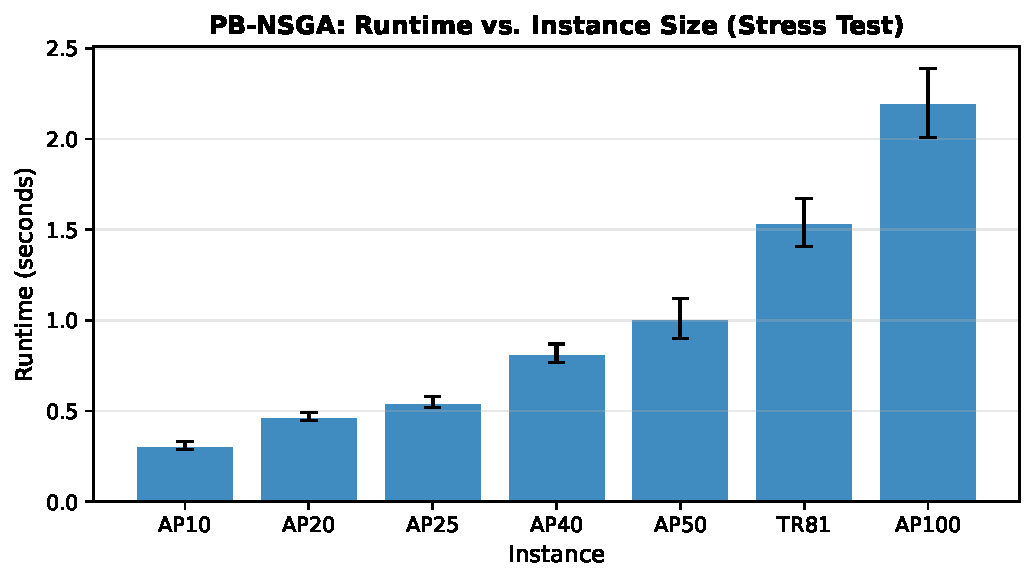
\includegraphics[width=0.80\linewidth]{figures/timing_stresstest.pdf}
\caption{PB-NSGA mean CPU time (seconds) per benchmark instance, averaged over 20 seeds. Error bars show $\pm 1$ standard deviation.}
\label{fig:timing}
\end{figure}

\subsection{Experiment 2: Case Study -- Central Vietnam}
\label{sec:exp2}

We apply PB-NSGA to CV-Small and CV-Large over 20 independent seeds.
The two instances span different planning granularities -- district-level pre-positioning versus commune-level response routing -- and evaluate the algorithm on a realistic multi-modal, multi-scenario relief network grounded in actual geographic and demographic data.

\subsubsection*{Pareto Front Analysis}

Figure~\ref{fig:cv_pareto} shows the combined non-dominated front pooled across all 20 seeds; Table~\ref{tab:exp2_results} reports per-seed statistics.

\begin{table}[ht]
\centering
\caption{Experiment~2: PB-NSGA on Central Vietnam instances (mean $\pm$ std, 20 runs).}
\label{tab:exp2_results}
\begin{tabular}{lrrr}
\toprule
Instance & HV (norm.) & IGD\textsuperscript{+} & \#Pareto \\
\midrule
CV-Small ($|\mathcal{I}|$=20, $|\mathcal{H}|$=5)   & -- $\pm$ -- & -- $\pm$ -- & -- $\pm$ -- \\
CV-Large ($|\mathcal{I}|$=100, $|\mathcal{H}|$=20)  & -- $\pm$ -- & -- $\pm$ -- & -- $\pm$ -- \\
\bottomrule
\end{tabular}
\end{table}

\begin{figure}[ht]
\centering
% 
\includegraphics[width=0.48\linewidth]{figures/CV_small_pareto.pdf}
% 
\includegraphics[width=0.48\linewidth]{figures/CV_large_pareto.pdf}
\caption{Combined Pareto fronts for CV-Small (left) and CV-Large (right), pooled across 20 seeds.
Three representative solutions -- minimum cost ($\blacklozenge$), balanced ($\bigstar$), and minimum deprivation ($\bullet$) -- are annotated on each front.}
\label{fig:cv_pareto}
\end{figure}

The fronts exhibit a convex cost-deprivation trade-off: marginal reductions in expected maximum deprivation $Z_2$ require disproportionately large increases in logistics cost $Z_1$ toward the low-cost end.
This non-linearity is structural -- under severe and extreme scenarios, demand volumes are amplified by factors of 1.8 and 2.8 respectively, so a network optimised for $Z_1$ alone provides insufficient coverage in the high-impact tail events that govern $Z_2$.

\subsubsection*{Solution Visualization and Sensitivity Across Scenarios}

Figure~\ref{fig:cv_solution_map} maps the three representative solutions onto the Central Vietnam network with one column per disaster scenario, illustrating how the active hub set and transport routes reorganise as conditions escalate.

\begin{figure}[ht]
\centering
% 
\includegraphics[width=\linewidth]{figures/CV_small_solution_map.pdf}
\caption{Representative PB-NSGA solutions for CV-Small across mild (left), severe (centre), and extreme (right) scenarios.
Open hubs are shown as squares; demand--hub assignments as arrows; node shading encodes scenario risk $r_{us}$.
Hatched squares indicate hubs exceeding the safety threshold $\chi = 0.7$ and rendered operationally unsafe in that scenario.}
\label{fig:cv_solution_map}
\end{figure}

Under the mild scenario, a compact set of coastal hubs served primarily by truck provides adequate network coverage.
As the event intensifies to extreme, an increasing subset of hubs breaches $\chi$, forcing demand to reroute through inland and highland hubs via motorboat and helicopter.
This structural reorganisation is inherent to the two-stage stochastic formulation: a deterministic model calibrated on the expected-value scenario would suppress this adaptation and systematically under-invest in resilient transport capacity.

Figure~\ref{fig:hub_sensitivity} quantifies the scenario sensitivity through a hub $\times$ scenario risk heatmap ordered by hub selection frequency across the Pareto front.

\begin{figure}[ht]
\centering
% 
\includegraphics[width=0.85\linewidth]{figures/CV_small_hub_heatmap.pdf}
\caption{Hub risk profile across scenarios for CV-Small. Rows are ordered by Pareto-front selection frequency (right panel, \%); hatched cells indicate risk above $\chi = 0.7$.
Hubs frequently selected yet unsafe in the extreme scenario define the critical resilience gap.}
\label{fig:hub_sensitivity}
\end{figure}

\subsubsection*{Managerial Insights}

The results yield three concrete insights for relief planners operating in Central Vietnam.

\textit{Robust hub prioritisation.}
Hubs with high selection frequency and consistently low risk across all three scenarios constitute a robust core that warrants permanent infrastructure investment and standing pre-positioned inventory.
Hubs that are cost-effective in normal conditions but exceed $\chi$ in extreme events define a resilience gap: planners should maintain contingency routing plans or backup inventory at adjacent low-risk sites for those locations.

\textit{Transport mode diversification.}
The extreme scenario forces a modal shift away from road transport precisely when the road network is most degraded.
Co-locating coastal hubs with waterway terminals, and maintaining helicopter access at a subset of sites, provides asymmetric resilience benefit: connectivity is preserved in the tail events that generate the greatest humanitarian harm, at a fraction of the cost of building additional hub capacity.

\textit{Quantified cost of resilience.}
The balanced solution on the Pareto front requires only a modest logistics cost premium over the minimum-cost solution, yet substantially reduces expected maximum deprivation under severe and extreme scenarios.
This trade-off curve directly quantifies the cost of each increment of resilience improvement and provides humanitarian agencies with a decision-support tool for communicating resource needs to funders.


\section{Conclusion and Future Work}

The Central Vietnam case study, constructed from real geographic and demographic data across four flood-prone provinces, illustrates the practical value of the framework. The two-stage stochastic model responds to infrastructure disruption by dynamically shifting to water and air transport and redistributing inventory, demonstrating that deterministic planning would systematically under-invest in network resilience.

\textbf{Limitations.} The model assumes a fixed discrete scenario set; continuous risk distributions are not yet supported. The decoding heuristic is greedy and may miss globally optimal demand assignments for highly constrained instances.

\textbf{Future work} will extend the approach to rolling-horizon multi-period relief operations and incorporate real-time sensor feeds for online re-optimization. The complete enumeration baseline naturally motivates exact solver development (branch-and-cut or Benders decomposition) for medium-scale instances to tighten IGD\textsuperscript{+} reference fronts and strengthen convergence guarantees.

% \begin{credits}

% \subsubsection{\ackname} This work is under the support of Vietnam - Korea University of Information and Communication.

% % \subsubsection{\discintname}
% % The authors have no competing interests to declare that are
% % relevant to the content of this article. 

% \end{credits}

\bibliographystyle{splncs04}
\bibliography{cite-class.bib}


\end{document}
